%%%%%%%%%%%%%%%%%%%%%%%%%%%%%%%%%%%%%%%%%%%%%%%%%%%%%%%%
%%%%%%%%%%%%%%%%%%%%%%%%%%%%%%%%%%%%%%%%%%%%%%%%%%%%%%%%
%%%%%%%%%%%%%%%%%%%%%%%%%%%%%%%%%%%%%%%%%%%%%%%%%%%%%%%%
\chapter{\sql}
\label{sql}

%%%%%%%%%%%%%%%%%%%%%%%%%%%%%%%%%%%%%%%%%%%%%%%%%%%%%%%%
%%%%%%%%%%%%%%%%%%%%%%%%%%%%%%%%%%%%%%%%%%%%%%%%%%%%%%%%
\section{Basic Commands (MySQL)}
\label{sql:basic}

\begin{lstlisting}[language=SQL]
-- create a new table, define columns & types
CREATE TABLE t (id INT PRIMARY KEY,
 name VARCHAR(20), state VARCHAR(2));

-- manually insert new rows
INSERT INTO t VALUES (0, 'Matt', 'NJ');
INSERT INTO t (id, name, state) VALUES (1, 'Jamie', 'NJ');
INSERT INTO t VALUES (2,'Marry','IL'), (3,'Eddie','IL'),
 (4,'Bob','ND'), (5,'Peter','MN');

-- insert rows from another table
INSERT INTO t SELECT * FROM other_t WHERE zip = 11111;

/* select with where, order by, limit
comparison ops: >, >=, =, <>, BETWEEN, LIKE, IN
logical ops: AND, OR, NOT */
SELECT id,name FROM t WHERE id > 0 ORDER BY name LIMIT 10;
SELECT id,name FROM t WHERE id BETWEEN 1 AND 3;
SELECT id,name FROM t WHERE name LIKE 'M\%';-- starts with M
SELECT id,name FROM t WHERE (id IN (0, 3)) OR (name = 'Bob');

-- select unique / distinct values
SELECT DISTINCT name FROM t;

-- finding nulls, use IS, NOT IS; can't use <>, =
SELECT id,name FROM t WHERE state IS NULL;

-- aggregation commands
SELECT count(1) AS 'nrows' FROM t;
SELECT count(id) FROM t WHERE id NOT IN (0, 1);
SELECT MIN(id) FROM t;
-- plus MAX, AVG, and SUM

-- GROUP BY
SELECT state,COUNT(id) FROM t GROUP BY state
 ORDER BY COUNT(id) DESC;

-- Use HAVING with an aggregate func, not WHERE
SELECT state,COUNT(id) FROM t GROUP BY state
 HAVING COUNT(id) > 5;

-- WITH / subqueries
WITH state_counts AS (
 SELECT count(id) AS 'count',state FROM t GROUP BY state )
SELECT AVG(count) FROM state_counts WHERE state <> 'NC';

-- update row
UPDATE t SET name = 'Mar' WHERE id = 2;

-- CASE
SELECT name,
  CASE
    WHEN state IS 'IL' THEN 'bears fan'
    WHEN state IS 'NC' THEN 'bison fan'
    ELSE CONCAT(name, ' (unknown)')
  END
FROM t;

-- return duplicate rows using a join
SELECT  t1.*, t2.totalCount AS Nduplicates
FROM    t t1
        INNER JOIN
        (
            SELECT  state, COUNT(*) totalCount
            FROM    t
            GROUP   BY state
            HAVING  COUNT(*) >= 2
        ) b ON a.state = b.state

-- Select the top 5 steam games per user, having a min of 120 minutes of playtime
SELECT steamid, appid, playtime_forever
 FROM
 (
   SELECT steamid, appid, playtime_forever,
   @steamid_rank := IF(@current_steamid = steamid,
                         @steamid_rank + 1,
                         1
                      ) AS steamid_rank,
   @current_steamid := steamid
   FROM Games_1
   WHERE playtime_forever > 120
   ORDER BY steamid, playtime_forever DESC
 ) ranked
 WHERE steamid_rank <= 5;
\end{lstlisting}
% For "select the top 5 steam games per user..." see https://www.databasejournal.com/features/mysql/selecting-the-top-n-results-by-group-in-mysql.html

% TODO renaming columns
% TODO change column types
% TODO possible types
% TODO dealing with dates?

%%%%%%%%%%%%%%%%%%%%%%%%%%%%%%%%%%%%%%%%%%%%%%%%%%%%%%%%
%%%%%%%%%%%%%%%%%%%%%%%%%%%%%%%%%%%%%%%%%%%%%%%%%%%%%%%%
\section{Joining}
\label{sql:join}
% TODO

\begin{figure}[H]
\centering
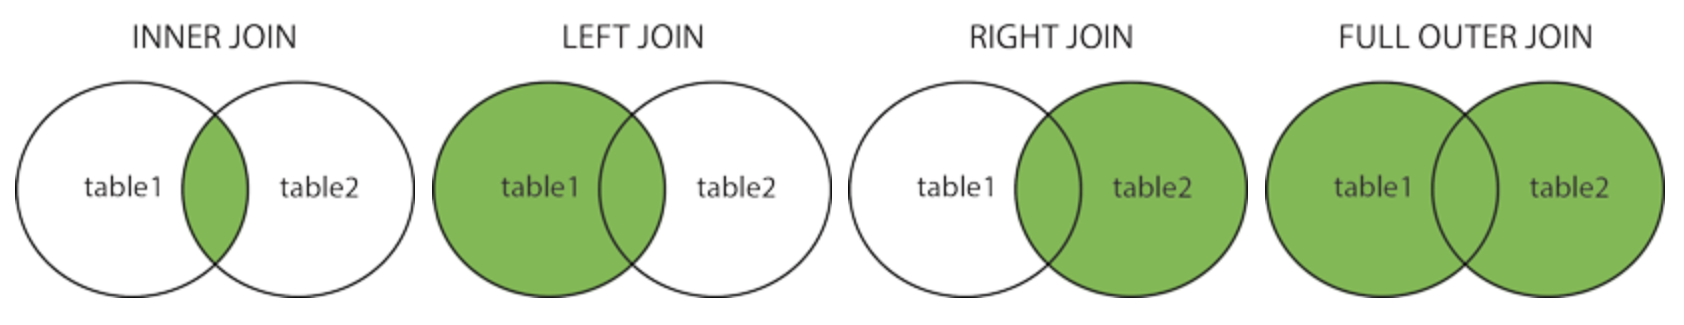
\includegraphics[width=0.8\textwidth]{figures/sql/joins.png}
\caption{
Illustration of the types of joins, by \href{https://www.w3schools.com/sql/sql_join.asp}{w3schools.com}.
}
\label{fig:sql:joins}
\end{figure}

%%%%%%%%%%%%%%%%%%%%%%%%%%%%%%%%%%%%%%%%%%%%%%%%%%%%%%%%
%%%%%%%%%%%%%%%%%%%%%%%%%%%%%%%%%%%%%%%%%%%%%%%%%%%%%%%%
\section{Pivoting}
\label{sql:pivoting}
% TODO

%%%%%%%%%%%%%%%%%%%%%%%%%%%%%%%%%%%%%%%%%%%%%%%%%%%%%%%%
%%%%%%%%%%%%%%%%%%%%%%%%%%%%%%%%%%%%%%%%%%%%%%%%%%%%%%%%
\section{IO Commands}
\label{sql:io}

\begin{lstlisting}[language=SQL]
-- admin, setup new user
GRANT ALL PRIVILEGES ON *.* TO 'user'@'localhost'
 IDENTIFIED BY 'pw';

-- create a new database
CREATE DATABASE mydb; USE mydb;

-- load a SQL dump
SET autocommit=0; SOURCE dump.sql; COMMIT;

-- load csv file into table
LOAD DATA LOCAL INFILE 'in.csv' INTO TABLE tnew
 FIELDS TERMINATED BY ',' LINES TERMINATED BY '\n';

-- delete a row, drop/add column, table, database
DELETE FROM t WHERE id = 4;

SHOW COLUMNS FROM t; /* or, also for MySQL */ DESCRIBE t;
SHOW COLUMNS FROM t WHERE Type LIKE 'Varchar\%';
ALTER TABLE t DROP COLUMN name;
ALTER TABLE t ADD weight DOUBLE;

SHOW TABLES;
DROP TABLE IF EXISTS 't';

SHOW DATABASES;
DROP DATABASE mydb;
\end{lstlisting}

\begin{lstlisting}[language=bash]
# export selection to csv (from shell, no file permissions)
mysql -u user --password=pw --database=mydb
 --execute='SELECT ...;' -q -n -B -r > o.csv
 && sed -i '/\t/ s//,/g' o.csv

# load table from csv (from shell)
mysqlimport --ignore-lines=1 --fields-terminated-by=,
 --verbose --local -u user -p mydb /path/to/in.csv
\end{lstlisting}
